\documentclass{beamer}
\mode<presentation> {
\usetheme{Boadilla}
}

%%import packages....I didnt use all of these, they're just in my template
\usepackage{graphicx}
\usepackage{booktabs}
\usepackage{standalone}
\usepackage{tikz}
\usepackage{textpos}
\usepackage{modiagram}
\usepackage{physics}
\usepackage{amsmath}
\usepackage[percent]{overpic}
\usepackage{subfig}
\usepackage{xcolor}
\usepackage{subfiles}
\usepackage{hyperref}



\usetikzlibrary{arrows.meta,positioning,decorations.markings,backgrounds}

\tikzset{
    every node/.style={font=\footnotesize},
}

%%citation style parameters

\usepackage[backend=bibtex,%
isbn=false,%
url=false,%
style=authoryear,%
% firstinits=false,
maxbibnames=2,%
]{biblatex}
\bibliography{My Collection.bib}

\renewbibmacro*{cite}{%
  \iffieldundef{shorthand}
    {\ifthenelse{\ifnameundef{labelname}\OR\iffieldundef{labelyear}}
       {\usebibmacro{cite:label}%
        \setunit{\printdelim{nonameyeardelim}}}
       {\printnames{labelname}%
        \setunit{\printdelim{nameyeardelim}}}%
     \usebibmacro{cite:labeldate+extradate}%
     \setunit{\addcomma\space}%
     \usebibmacro{journal}}
    {\usebibmacro{cite:shorthand}}}



%I dont remember why I have this in my template
\usetikzlibrary{decorations.pathreplacing,angles,quotes}

%%UNT color scheme
\colorlet{beamer@blendedblue}{green!40!black}

% Title Information
\title[LIBS]{LIBS of Sputtering Targets}
\author{Brian Squires}
\institute[UNT]
{
University of North Texas \\
\medskip
\textit{Department of Physics}\\
\medskip
\textit{brian.squires@unt.edu}\\
\medskip
\textit{}
}
\date{\today}
% \logo{\vspace{7.25cm}\includegraphics[height=1.5cm]{/Users/briansquires/github/logo1.jpg}}

%Add shaded outline slide before each section
\AtBeginSection[]
{
    \begin{frame}
        \frametitle{Outline}
        \tableofcontents[currentsection]
    \end{frame}
}


\begin{document}
\begin{frame}
    \titlepage    
\end{frame}

% \begin{frame}
%     \includegraphics[scale=0.5, angle=-90]{/Users/briansquires/Documents/LIBS/IMG_1921.HEIC.pdf}
% \end{frame}

% \begin{frame}{Average Linewidth = 0.9996nm}
%     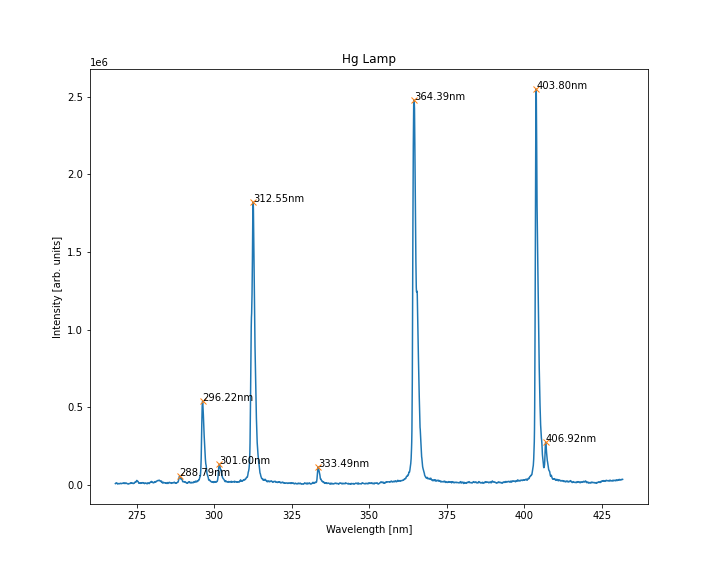
\includegraphics[scale=0.45]{calibrationlamp.png}
% \end{frame}

\foreach \x in {Al, Bi, Co, Cr, Fe, Hf, In, Nb, Ru, V, Y, Zn, Zr}
{    \begin{frame}
        \includegraphics[scale=0.5]{/Users/briansquires/Documents/LIBS/data/20211026/Sputtering Targets/elements_350nm/\x.png}
    \end{frame}
}

\foreach \x in {Al2O3(2)ZnO(98), BN, HfC, Inconel, ITO, MoS2, Ni3Al, NiV, TaC, ZnO}
{    \begin{frame}
        \includegraphics[scale=0.5]{/Users/briansquires/Documents/LIBS/data/20211026/Sputtering Targets/binary_350nm/\x.png}
    \end{frame}
}

\foreach \x in {350nm, 450nm, 550nm}
{    \begin{frame}{Fe Argon/Air Test}
        \begin{columns}
            \begin{column}{0.5\textwidth}
                 \includegraphics[scale=0.25]{/Users/briansquires/Documents/LIBS/data/20220705/air_\x.png}
            \end{column}
            \begin{column}{0.5\textwidth}
                \includegraphics[scale=0.25]{/Users/briansquires/Documents/LIBS/data/20220705/argon_\x.png}
            \end{column}
        \end{columns}
    \end{frame}
}


\foreach \x in {Al, BN, C, Cr, Cu, Fe, Inconel, Ni, TiO2, W, Zn, ZnO}
{    \begin{frame}
        \includegraphics[width=\textwidth]{/Users/briansquires/Documents/LIBS/data/20220705/\x/\x.png}
    \end{frame}
}

\begin{frame}
    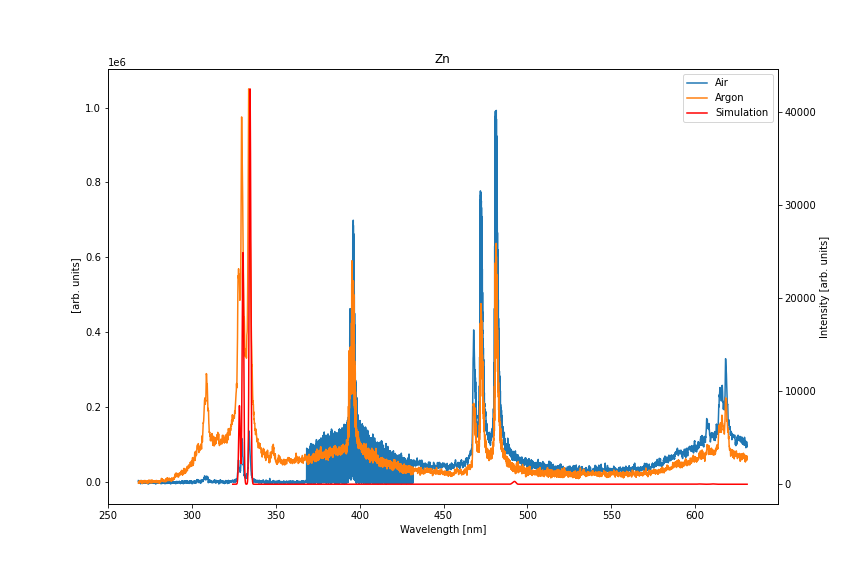
\includegraphics[width=\textwidth]{/Users/briansquires/Documents/LIBS/data/20220706/Zn/Zn.png}
\end{frame}

\begin{frame}
    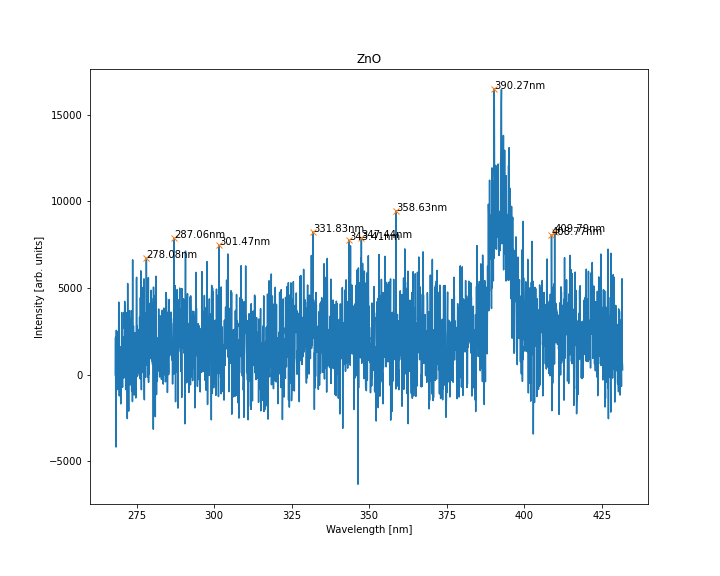
\includegraphics[width=\textwidth]{/Users/briansquires/Documents/LIBS/data/20220706/ZnO/ZnO.png}
\end{frame}

\begin{frame}
    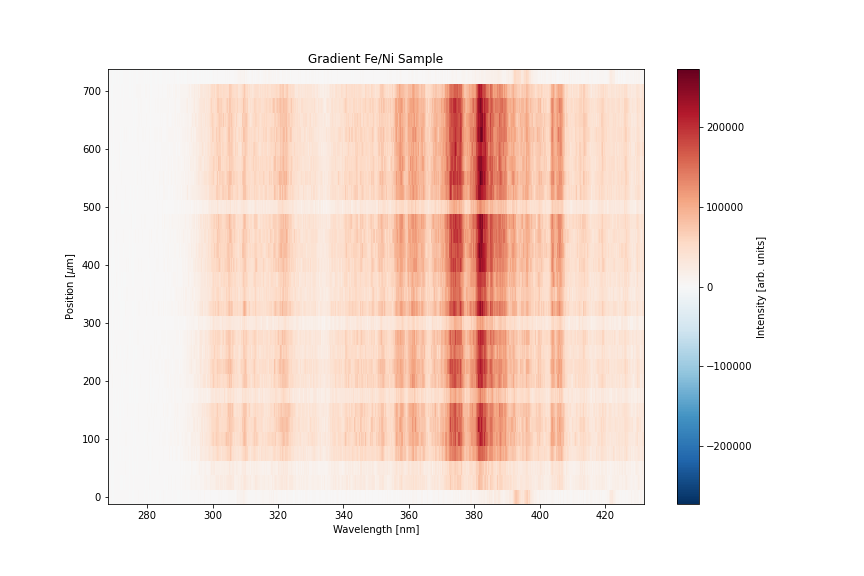
\includegraphics[width=\textwidth]{/Users/briansquires/Documents/LIBS/data/20220705/gradient_sample/gradient_sample.png}
\end{frame}

\begin{frame}
    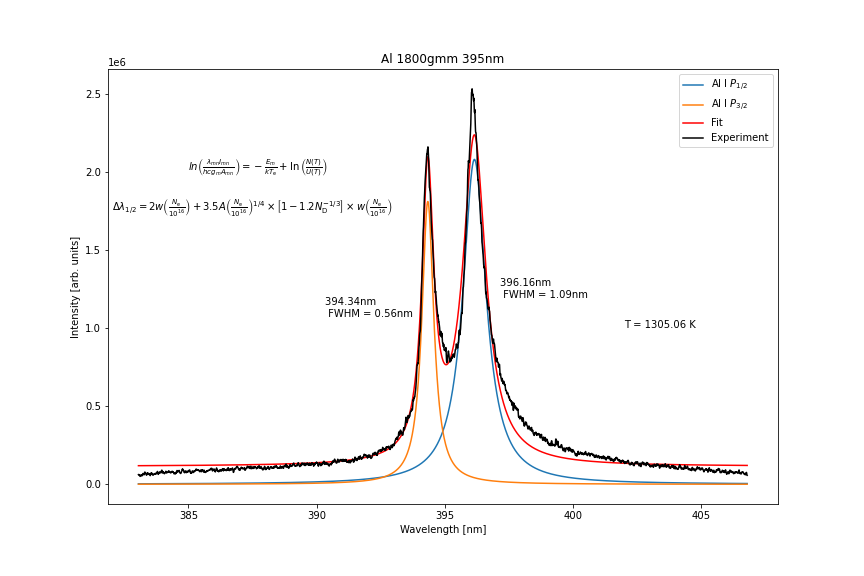
\includegraphics[width=\textwidth]{/Users/briansquires/Documents/LIBS/LorentzFit_Al.png}
\end{frame}

\begin{frame}{Other}
    \begin{itemize}
        \item Optical Path Rebuild
        \begin{itemize}
            \item Replaced mirrors with dual wavelength dielectric high reflectors
            \item Replaced collection lens with UV enhanced achromatic doublet
        \end{itemize}
    \end{itemize}
\end{frame}

\end{document}